\subsubsection{API Gateway trong Microservice (Kong API Gateway)}

API Gateway
được sử dụng
để quản lý
và kiểm soát việc truy cập vào các API.
API Gateway cung cấp một lớp trung gian
giữa client và các dịch vụ.
Có thể nói, API Gateway
là một điểm vào độc lập cho nhiều client của một ứng dụng.
Kong API Gateway
là một trong những API Gateway
mã nguồn mở
phổ biến
có thể quản lý
các API được triển khai ở bất kỳ đâu,
từ cơ sở hạ tầng đơn giản đến môi trường đa đám mây phức tạp.

\begin{figure}[H]
\centering
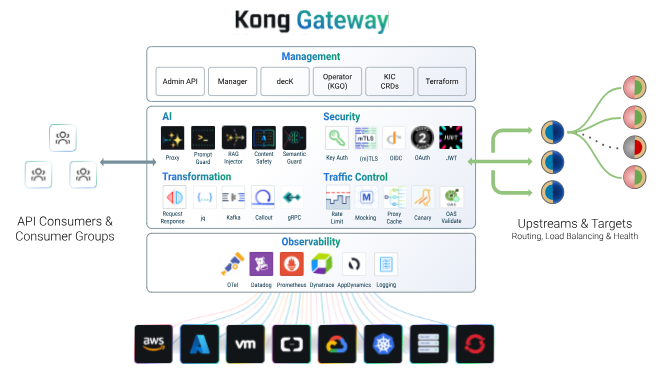
\includegraphics[width=0.8\textwidth]{pictures/kong-gateway-overview.excalidraw.png}
\caption[Sơ đồ tổng quan kiến trúc và luồng hoạt động của Kong API Gateway]{Sơ đồ tổng quan kiến trúc và luồng hoạt động của Kong API Gateway (Nguồn: \cite{kong-gateway})}
\end{figure}

Trong
môi trường sản xuất thực tế
gặp nhiều thách thức, khó khăn.
Sử dụng các plugin của Kong như
rate limit giới hạn tốc độ yêu cầu,
bot-detection ngăn chặn các yêu cầu độc hại.

\begin{figure}[H]
\centering
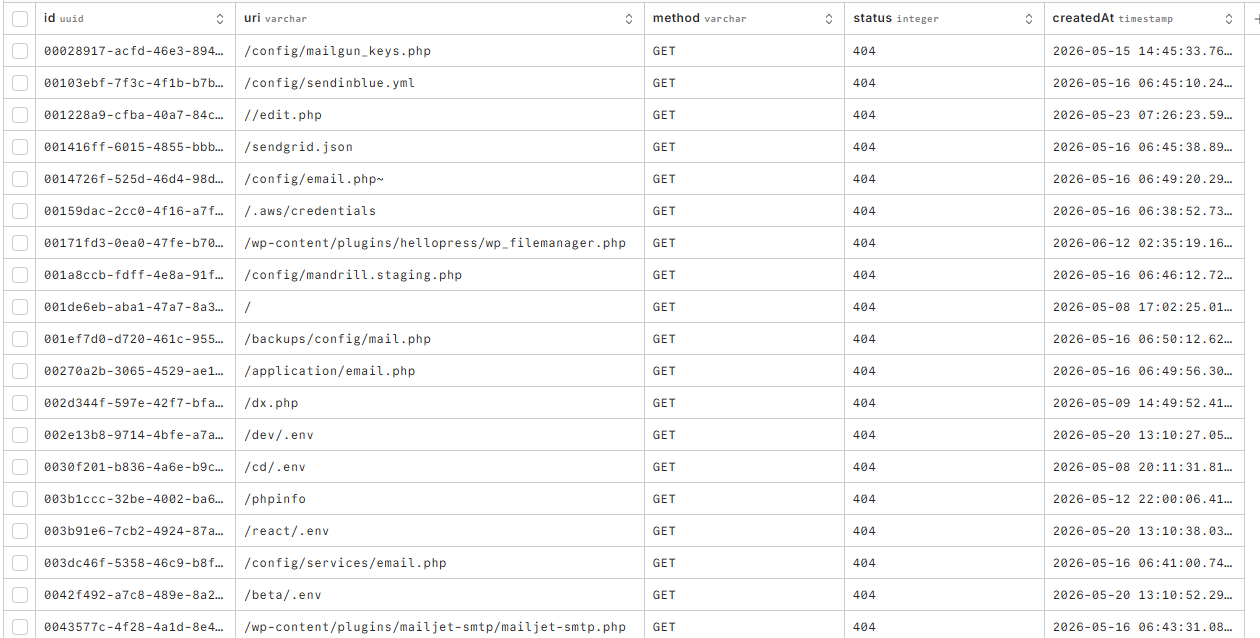
\includegraphics[width=0.7\textwidth]{pictures/kong-api-gateway-env-secret.png}
\caption{Các yêu cầu độc hại hacker dò các bí mật nhạy cảm (404 Not Found)}
\end{figure}
Cấu trúc dự án Kong API Gateway

\begin{figure}[H]
\centering
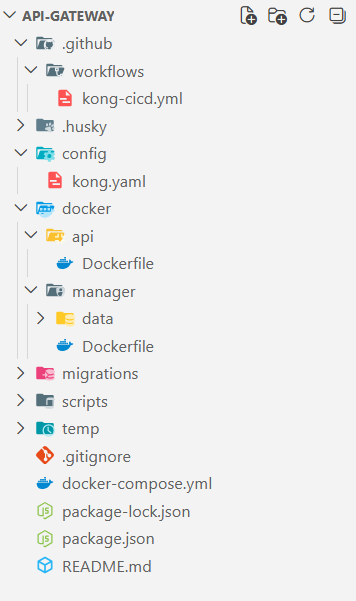
\includegraphics[width=0.5\textwidth]{pictures/kong-api-gateway-project-v2.png}
\caption{Cấu trúc dự án Kong API Gateway}
\end{figure}

\begin{figure}[H]
\centering
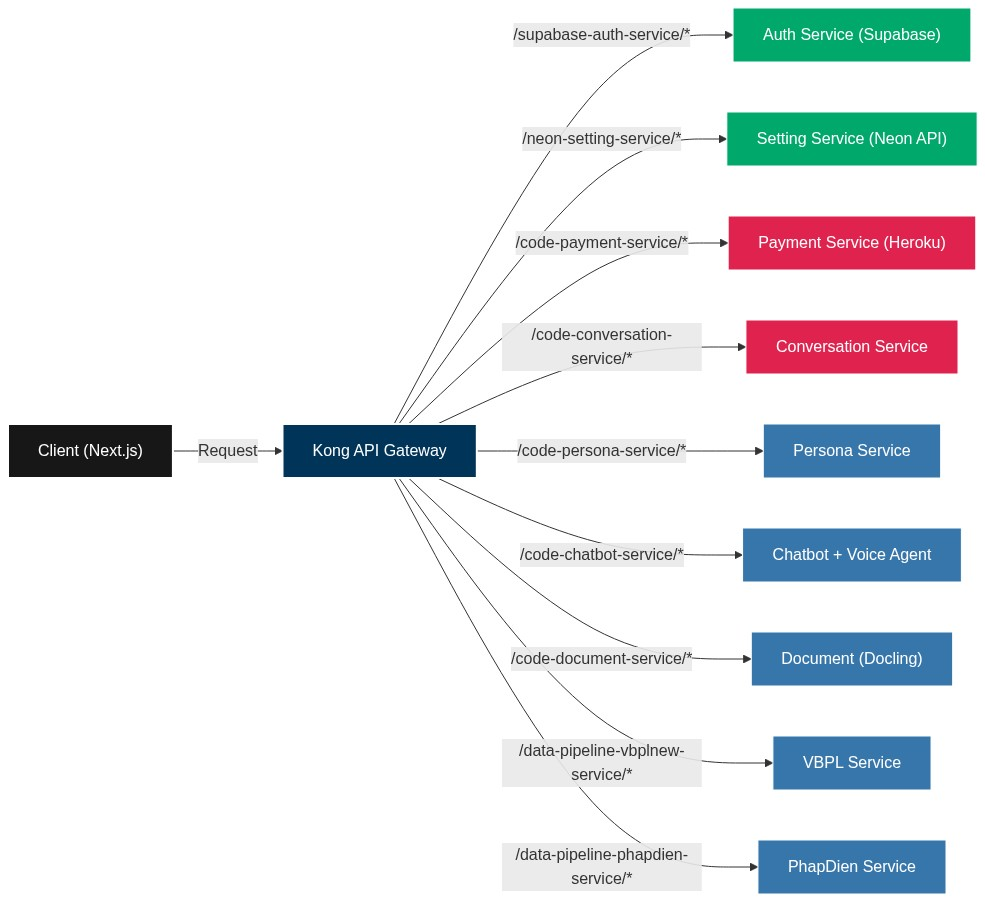
\includegraphics[width=0.7\textwidth]{pictures/kong-api-gateway-router.png}
\caption{Thiết lập định tuyến dịch vụ trong Kong API Gateway}
\end{figure}

Kong API Gateway
có hỗ trợ
nhiều cách quản lý
cấu hình khác nhau như
Kong Admin API (REST API), Terraform hay qua các giao diện UI.
Tuy nhiên, Deck lại là công cụ được chính Kong
phát triển để tối ưu hóa riêng cho việc quản lý cấu hình.
Với Terraform,
nếu ai đó vào giao diện hoặc gọi REST API
sửa đổi một cấu hình của Kong, file terraform.tfstate sẽ bị lệch,
dẫn đến việc apply tiếp theo có thể lỗi hoặc đè dữ liệu.
Với Deck sẽ đọc trực tiếp cấu hình hiện tại trong database của Kong,
so sánh (diff) với file YAML
và chỉ cập nhật những phần thay đổi qua API dạng batch tối ưu.
Không sợ bị lệch trạng thái.
Ngoài ra, Deck hỗ trợ CI/CD với GitHub Actions (kong/setup-deck).
Lưu trữ toàn bộ cấu hình Kong API Gateway
với file kong.yaml vào một kho chứa Git
Thiết lập các pipeline
để tự động kiểm tra cú pháp deck gateway validate kong.yaml,
tự động so sánh thay đổi deck gateway diff kong.yaml
và tự động cập nhật deck gateway sync kong.yaml
khi có Pull Request được merge.

\begin{figure}[H]
\centering
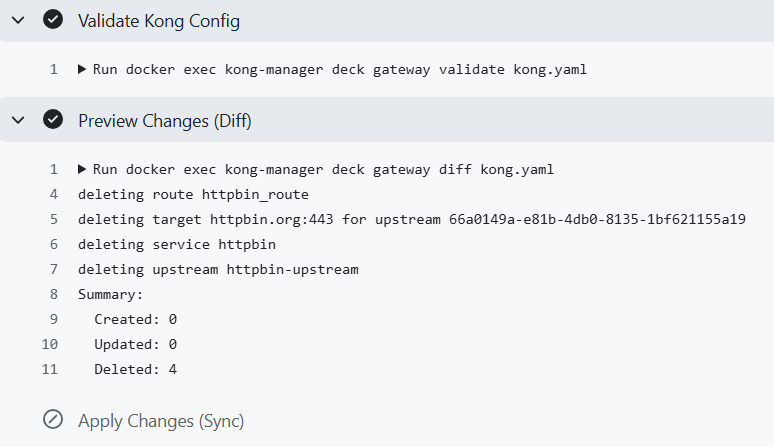
\includegraphics[width=0.95\textwidth]{pictures/kong-api-gateway-github-action-v2.png}
\caption{Luồng CI/CD triển khai cấu hình Kong API Gateway qua GitHub Actions}
\end{figure}

\begin{figure}[H]
\centering
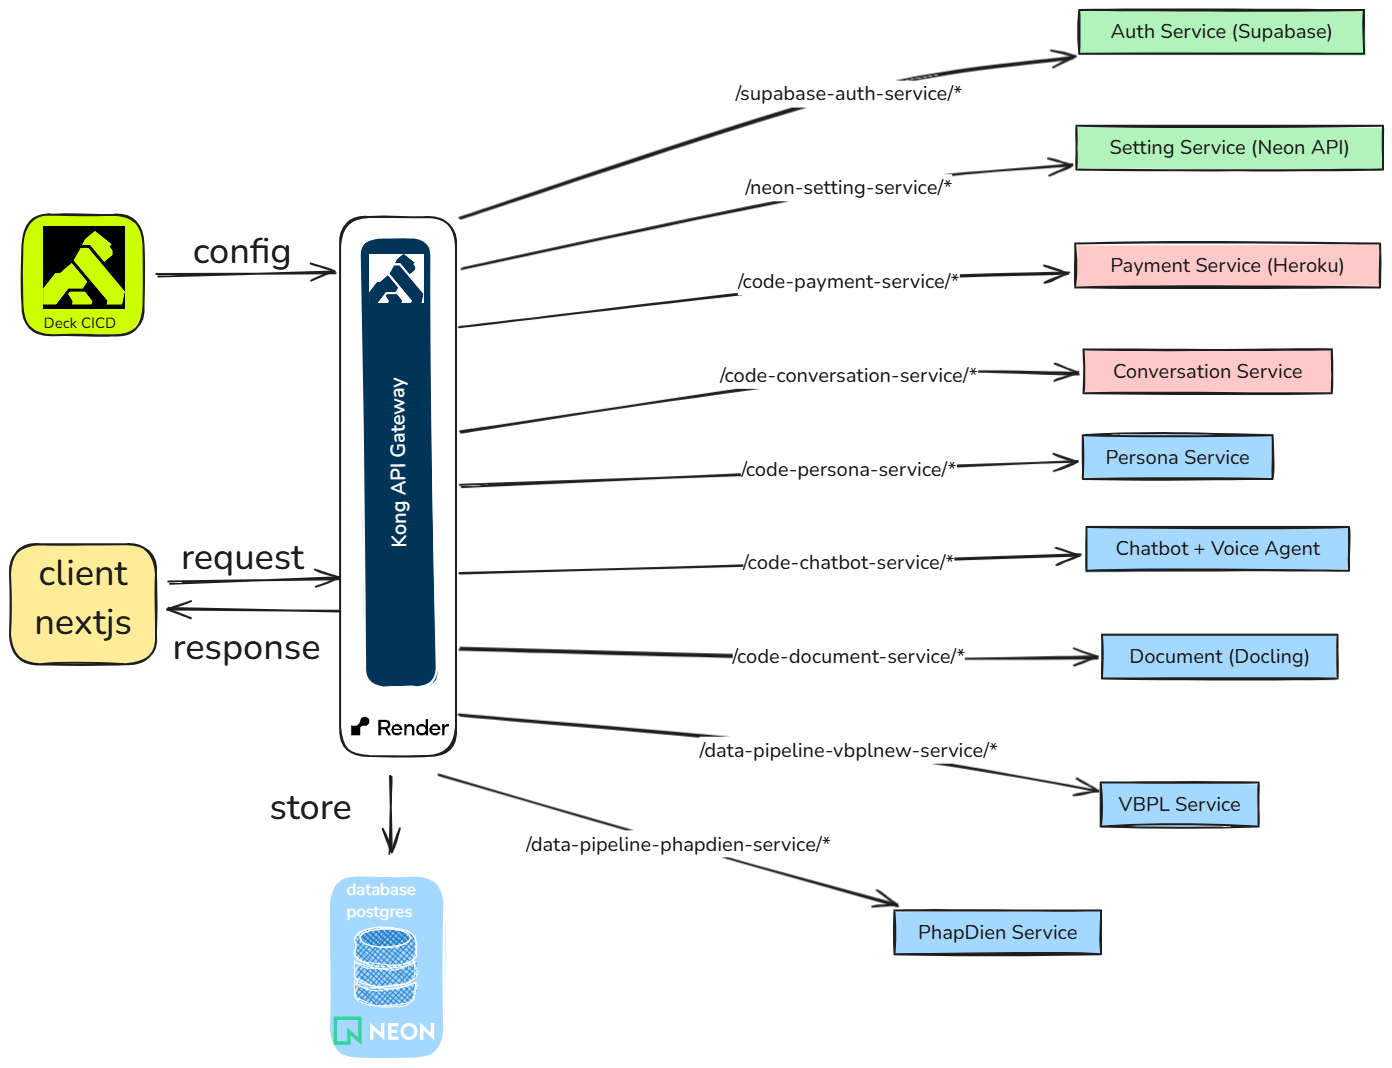
\includegraphics[width=0.7\textwidth]{pictures/request-response-result-Kong-API-Gateway.excalidraw.png}
\caption{Sử dụng Deck và database postgres cấu hình Kong API Gateway}
\end{figure}

Các plugins của Kong API Gateway trong dự án này:

\begin{itemize}
\item Plugin bot-detection: phân tích User-Agent và các dấu hiệu khác để chặn các yêu cầu từ các bot độc hại, scraper, hoặc các công cụ tự động không mong muốn.

\item Plugin rate-limiting: giới hạn số lượng yêu cầu, giúp bảo vệ các dịch vụ khỏi bị quá tải hoặc bị lạm dụng.

\item Plugin request-size-limiting: chặn các yêu cầu có kích thước vượt quá ngưỡng cho phép.

\item Plugin http-log: thu thập các thông tin quan trọng về request/response và gửi qua giao thức http api NestJS và thực hiện lưu vào database postgres

\item Plugin correlation-id tạo request-id: tự động tạo ra một mã định danh duy nhất và gắn vào header của mỗi yêu cầu để truy vết (tracing).

\item Plugin request-transformer thêm thông tin Request-Kong-Secret: gửi header chứa mã bí mật vào yêu cầu trước khi đẩy xuống dịch vụ để các yêu cầu phải được gọi từ Kong API Gateway.
\end{itemize}

\begin{figure}[H]
\centering
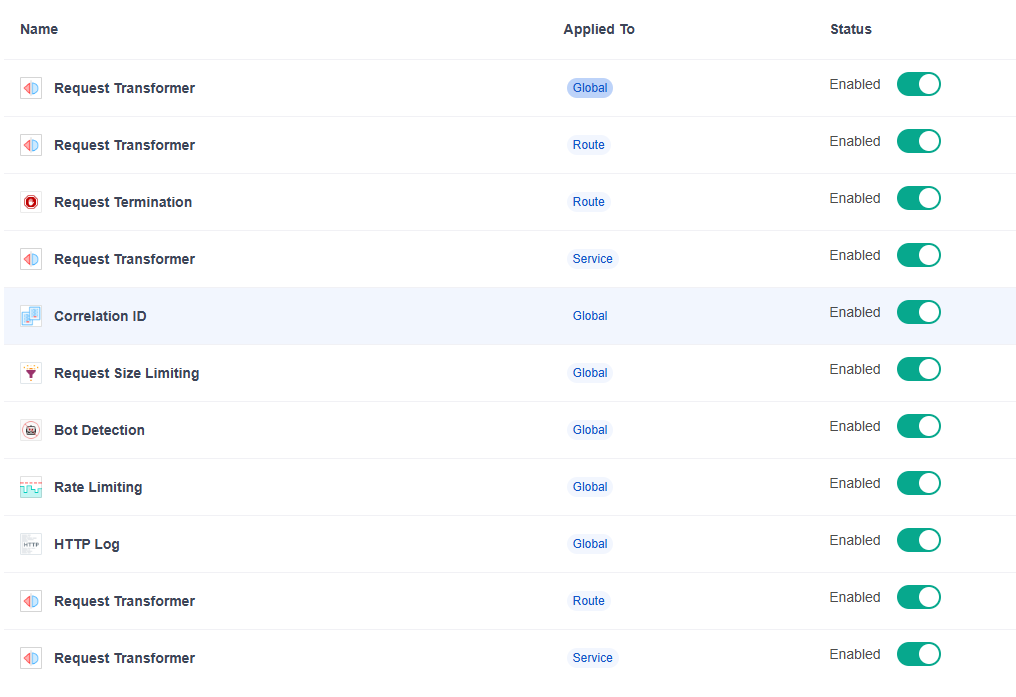
\includegraphics[width=0.95\textwidth]{pictures/kong-api-gateway-plugin.png}
\caption{Danh sách các plugin được cấu hình trên Kong API Gateway}
\end{figure}

Các kết quả phản hồi Kong API Gateway:

\begin{figure}[H]
\centering
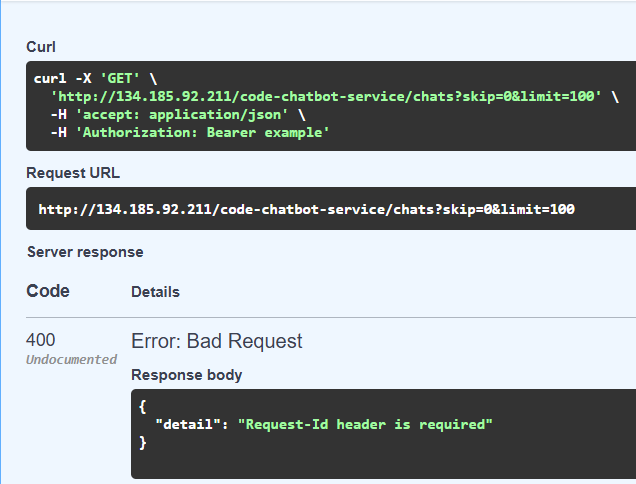
\includegraphics[width=0.6\textwidth]{pictures/kong-api-gateway-request-id-not.png}
\caption{Phản hồi khi yêu cầu thiếu mã định danh Request ID}
\end{figure}

\begin{figure}[H]
\centering
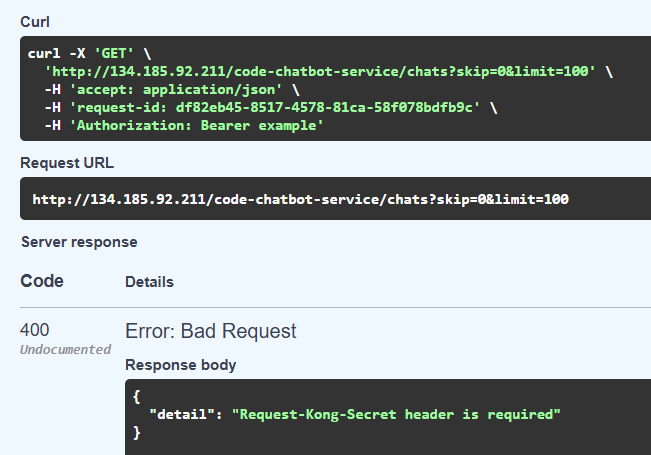
\includegraphics[width=0.95\textwidth]{pictures/kong-api-gateway-request-kong-secret-not.png}
\caption{Phản hồi khi yêu cầu thiếu mã bảo mật Kong Secret}
\end{figure}

\begin{figure}[H]
\centering
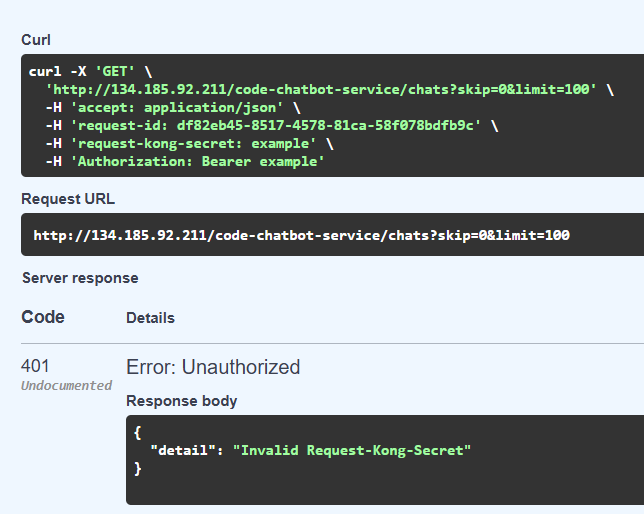
\includegraphics[width=0.95\textwidth]{pictures/kong-api-gateway-request-kong-secret-invalid.png}
\caption{Phản hồi khi mã bảo mật Kong Secret không hợp lệ}
\end{figure}
